
\section{Alexander-Spanier \trCohomology{}的连续性}
\label{sec:alexander-spanier-continuity}

\hzsync{definition}{1}%
\hzsync{theorem}{13}%
\hzsync{proposition}{8}%
\hzsync{corollary}{1}%
\hzsync{equation}{51}%

第 6 章所需的数学工具正在变得更加精深。特别地，\trHomology{}与%
\trCohomology{}理论正在被使用。除了（上）\trHomology{}理论的基本性质之外，%
读者还需要了解\trCupProduct{}与\textbf{\trPoincare\trDual{}性}（Poincaré duality）。%
所有这些内容都可以在\textbf{\trAlgebraicTopology}（algebraic topology）的标准教科书
中找到。我们推荐，例如，J.~\trn{Vick}{维克}的书 [216]，它非常仔细地描述了
标准材料，并且还提供了\trFixedPoint{}理论的介绍，引入了与\trDegree{}理论
密切相关的\textbf{\trFixedPointIndex}（fixed point index）。更全面的\trAlgebraicTopology{}论述
见于 A.~\trDold{} [62]、W.\,S.~\trMassey{} [148, 149, 150]、E.~\trSpanier{} [203]
以及 R.~\trn{Switzer}{斯威策} [209] 的著作。特别地，[62] 中关于%
\trHomotopyInvariant{}\trFunctor{}的 Kan 延拓与 \trCech{}延拓的附录，对下文关于%
\trHomotopyInvariant{}\trFunctor{}的连续性的讨论是有趣的。

非线性分析——有些夸张地说——就是对形如
\[F(x)\ =\ y\,.
\]
的非线性方程的研究。若映射 $F\colon X\to Y$ 以及\trTopology{}空间 $X$ 与 $Y$%
具有某些良好的性质，例如存在某种\trCompact{}性，且解集在\trGeneric{}的%
情形下是离散的，则\trDegree{}理论便是一个十分强大的工具。然而有时，人们%
期望解集在\trGeneric{}的情形下是\trManifold，当然也就想知道它们究竟是%
什么。一般而言这是一项困难的任务。但是，人们可以尝试利用%
\trHomology{}理论来计算它们的某些\trInvariant{}量。
于是，以下情形便相当频繁地出现。若我们考虑方程 $F(x)=y$，%
则对给定的 $y$，我们并不知道它是否落在\trGeneric{}的情形之中，从而解集%
可能行为相当糟糕，例如，它可能不是一个\trManifold。另一方面，可以选取%
\trGeneric{}的 $y_{k}$（即处于一般位置的值，例如\trRegular{}值），使得诸解集%
 $F^{-1}(y_{k})$ 表现良好，例如，它们是\trManifold，并用诸解集%
 $F^{-1}(y_{k})$ 来\trApproximation{}解集 $F^{-1}(y)$。在这种情形下，%
有时只能借助代数手段（利用\trHomology{}理论）来
研究 $F^{-1}(y_{k})$，于是问题便变成：在何种条件下我们能够对
$F^{-1}(y)$ 得出某种结论？

重要的工具将是\trHomology{}理论的\trContinuity，我们在下面
加以讨论。我们从适用于许多情形的抽象讨论开始，然后聚焦于我们在第 6 章
所需要的特定理论，即 \trAlexander-\trSpanier{}\trCohomology{}理论，参见
E.~\trSpanier{} [203]。

设 $X$ 是一个\trTopology{}空间，$\mathcal{C}$ 是一切子空间的\textbf{\trCategoryTheory}（category），
其\textbf{\trMorphism}（morphism）$\varphi\colon A\to B$ 是连续\trMapping。
设 $\mathcal{A}$ 是一个\textbf{\trAlgebraicCategory}（algebraic category）。我们考虑以下
情形之一：$\mathcal{A}$ 是\trAbelian{}群\trCategoryTheory，或是交换环\trCategoryTheory，或是某个
固定环上模的\trCategoryTheory。假设给定了一个\textbf{\trContravariant\trFunctor}（contravariant functor）
$h\colon\mathcal{C}\to\mathcal{A}$，即：对每个 $A\in\mathcal{C}$ 我们关联一个\textbf{\trAlgebraicObject}（algebraic
object）$h(A)\in\mathcal{A}$，而对每个连续\trMapping{}$\varphi\colon A\to B$ 我们关联一个%
\trHomomorphism $\varphi^{*}=h(\varphi)\colon h(B)\to h(A)$。若 $A\subset B$，则有一个自然的%
\trInclusionMapping，我们把它诱导的映射记作 $i_{AB}\colon h(B)\to h(A)$。
由于 $h$ 是一个\trContravariant\trFunctor，我们有
\[i_{AB}\,i_{BC}\ =\ i_{AC}\quad\text{对 }A\subset B\subset C
\]
\[i_{AA}\ =\ \operatorname{Id}_{h(A)}\,.
\]

给定 $A\subset X$，我们把 $A$ 的一切开\trNeighborhood{}的全体记作
$\mathcal{O}_{A}$。对 $U\in\mathcal{O}_{A}$，我们把由包含 $A\subset U$ 诱导的%
\trHomomorphism{}记作 $i_{U}\colon h(U)\to h(A)$。

\begin{definition}\label{def:a8-continuity}
设 $h$ 如上所述，$A\subset X$ 固定。我们称 $h$ 在 $A$ 处\textbf{连续}（continuous），
如果以下条件成立：
\begin{enumerate}
\item[(i)] 给定 $\alpha\in h(A)$，存在 $U\in\mathcal{O}_{A}$ 与
$\alpha_{U}\in h(U)$ 使得 $i_{U}(\alpha_{U})=\alpha$。
\item[(ii)] 给定 $\alpha_{U}\in h(U)$（$U\in\mathcal{O}_{A}$）满足
$i_{U}(\alpha_{U})=0$，则存在 $V\in\mathcal{O}_{A}$ 满足 $A\subset V\subset U$
且 $i_{VU}(\alpha_{U})=0$。
\end{enumerate}
\end{definition}

换言之，$h(A)$ 的每个元素 $\alpha$ 已经活在 $A$ 的某个\trNeighborhood{}
上，而每个在 $A$ 上「消亡」的类 $\alpha\in h(U)$（$U\in\mathcal{O}_{A}$）
已经在某个\trNeighborhood{}上「消亡」。

正如我们将在下文看到的，只要 $h$ 在 $A$ 处连续，我们便能从 $h(U)$
（$U\in\mathcal{O}_{A}$）重建 $h(A)$。

注意到 $\mathcal{O}_{A}$ 在以下意义上是一个\trDirectedSet。我们可以定义一个
序结构 $\leq$ 为
\[U\leq V\ :\Longleftrightarrow\ U\supset V
\]
（「更小的集合更大」）。此外，给定 $U$，$V\in\mathcal{O}_{A}$，存在
$W\in\mathcal{O}_{A}$ 满足
\[W\geq U\,,\qquad W\geq V\,.
\]

事实上，只须取 $W=U\cap V$。于是我们具有下述结构。对 $U\leq V$，有一个%
\trHomomorphism
\[i_{VU}\colon h(U)\longrightarrow h(V)
\]
而对每个 $U\in\mathcal{O}_{A}$ 有一个\trHomomorphism
\[i_{U}\colon h(U)\longrightarrow h(A)\,.
\]
此外，以下成立：若 $U\leq V\leq W$，则
\[i_{WV}\,i_{VU}\ =\ i_{WU}\qquad\text{且}\qquad i_{UU}=\operatorname{Id}\,.
\]
此外，若 $U\leq V$，则
\[i_{V}\,i_{VU}\ =\ i_{U}\,.
\]

我们首先执行一个称为\trDirectedLimit{}的构造，然后证明：只要 $h$ 在 $A$
处连续，它便与 $h(A)$\trIsomorphic。

定义 $M_{A}\in\mathcal{A}$ 为直和
\[M_{A}\ =\ \bigoplus_{U\in\mathcal{O}_{A}}h(U)\,.
\]
若 $\mathcal{A}$ 由\trAbelian{}群组成，则 $M_{A}$ 也是一个\trAbelian{}群，等等。
把包含到第 $U$ 个分量的\trHomomorphism{}记作 $\varphi_{U}$：
\[\varphi_{U}\colon h(U)\longrightarrow M_{A}\,.
\]

考虑由形如
\[\varphi_{U}(\alpha_{U})\ -\ \varphi_{V}\,i_{VU}(\alpha_{U})
\]
的元素生成的子群、理想或子模 $K_{A}$\footnote{原书印作「the subgroup, subring or submodule $K_{A}$」（子群、子环或子模），其「subring」欠确：子环上的商一般不再是环，唯取由这些关系元素生成的理想，商 $M_{A}/K_{A}$ 方能承袭环结构，故交换环情形应为「理想」，此处径改。——译者注}，其中 $U$，$V\in\mathcal{O}_{A}$ 满足
$U\leq V$，$\alpha_{U}\in h(U)$。定义
\[L_{A}\ =\ M_{A}/K_{A}\,.
\]

视 $\mathcal{A}$ 而定，这个\trQuotient{}或者是\trAbelian{}群，或者是交换环，
或者是模。

$L_{A}$ 的元素是等价类 $[(\alpha_{U})]$，其中 $(\alpha_{U})\in M_{A}$，%
$\alpha_{U}\neq0$ 至多对有限个 $U$ 成立（除有限多项外 $\alpha_{U}$ 皆为 $0$）。%
若 $\alpha_{U_{1}}$，$\ldots$、$\alpha_{U_{k}}$
是非零元素，则
\[(\alpha_{U})\ =\ \sum_{i=1}^{k}\varphi_{U_{i}}(\alpha_{U_{i}})\,.
\]

令 $U_{\infty}=\bigcap_{i=1}^{k}U_{i}$。任取 $V\in\mathcal{O}_{A}$，$V\geq U_{\infty}$。
则对 $i=1$，$\ldots$，$k$，
\[\beta_{i}\ :=\ \varphi_{U_{i}}(\alpha_{U_{i}})\ -\ \varphi_{V}\,i_{VU_{i}}(\alpha_{U_{i}})
\]
属于 $K_{A}$。于是
\[(\alpha_{U})\ =\ \sum_{i=1}^{k}\beta_{i}\ +\ \varphi_{V}\!\Big(\sum_{i=1}^{k}i_{VU_{i}}(\alpha_{U_{i}})\Big)
\ =:\ \beta\ +\ \varphi_{V}(\gamma)\,,
\]
其中 $\beta\in K_{A}$，$\gamma\in h(V)$。因此，对每个类 $a\in L_{A}$，
存在 $U_{a}\in\mathcal{O}_{A}$，使得对每个 $V\geq U_{a}$，$a$ 可以被
$\varphi_{V}(\alpha_{V})$ 表示，其中 $\alpha_{V}\in h(V)$ 是某个适当的元素。

对 $(\alpha_{U})\in M_{A}$，我们考虑元素
\[\hat{\Phi}\bigl((\alpha_{U})\bigr)\ :=\ \sum_{U\in\mathcal{O}_{A}}i_{U}(\alpha_{U})\ \in\ h(A)\,.
\]
注意这个和是有限的。对于元素
\[\beta\ =\ \varphi_{U}(\alpha_{U})\ -\ \varphi_{V}\,i_{VU}(\alpha_{U})\,,
\]
其中 $V\geq U$，我们计算：
\begin{align*}
\hat{\Phi}(\beta)\ &=\ i_{U}(\alpha_{U})\ -\ i_{V}\,i_{VU}(\alpha_{U})\\
&=\ i_{U}(\alpha_{U})\ -\ i_{U}(\alpha_{U})\\
&=\ 0\,.
\end{align*}
显然 $\hat{\Phi}\colon M_{A}\to h(A)$ 定义了一个\trHomomorphism。由前面的讨论，其%
\trKernel{}包含 $K_{A}$。于是我们得到一个\trHomomorphism
\[\Phi\colon L_{A}\longrightarrow h(A)\,.
\]

在精确的意义上，$\Phi$ 告诉我们 $h(U)$（$U\in\mathcal{O}_{A}$）对 $h(A)$
了解到了什么。上述构造是众所周知的\trDirectedLimit，记作
\[\check{h}(A)\ :=\ L_{A}\ =\ \operatorname*{dir.\,lim}_{\,U\in\mathcal{O}_{A}}\ h(U)\,.
\]
它是\trNeighborhood{}们相对于\trContravariant\trFunctor $h$ 对 $A$ 了解到了什么的一个
代数量度。

\begin{theorem}\label{thm:a8-direct-limit-isomorphism}
假设 $h$ 在 $A$ 处连续。则
\[\Phi\colon \check{h}(A)\longrightarrow h(A)
\]
是\trIsomorphic。
\end{theorem}

\begin{proof}
假设 $\Phi(a)=0$。由前面的讨论，我们可以用一个元素
$\varphi_{V}(\alpha_{V})$ 来表示 $a\in\check{h}(A)$，其中 $V\geq U_{a}$，
$\alpha_{V}\in h(V)$。于是
\[0\ =\ \Phi(a)\ =\ i_{V}(\alpha_{V})\,.
\]
由连续性定义的性质 \textup{(ii)}，我们找到 $W\geq V$ 使得
\[\alpha_{W}\ :=\ i_{WV}(\alpha_{V})\ =\ 0\,.
\]
注意
\begin{align*}
\varphi_{V}(\alpha_{V})\ &=\ \varphi_{V}(\alpha_{V})\ -\ \varphi_{W}\,i_{WV}(\alpha_{V})\\
&=\ \varphi_{V}(\alpha_{V})\ -\ \varphi_{W}(\alpha_{W})
\end{align*}
属于 $K_{A}$。因此 $a=0$。接下来设 $\beta\in h(A)$。由性质 \textup{(i)}，
存在 $U\in\mathcal{O}_{A}$ 与 $\alpha_{U}\in h(U)$ 使得 $i_{U}(\alpha_{U})=\beta$。
令 $a=[\varphi_{U}(\alpha_{U})]$。则 $\Phi(a)=\beta$。
\end{proof}

接下来假设 $h$ 是\trTopology{}空间\trCategoryTheory{}上的一个\trContravariant\trFunctor。设 $X$ 与 $A$ 如前，
并设 $Y$ 是另一个\trTopology{}空间。若 $f\colon X\to Y$ 是一个连续\trMapping，
我们想要研究 $f|_{A}\colon A\to Y$，并且一旦我们能够对 $f|_{U}\colon U\to Y$
（$U\in\mathcal{O}_{A}$）研究它的性质，便能对 $f|_{A}$ 的性质有所断言。
我们有交换图
\[
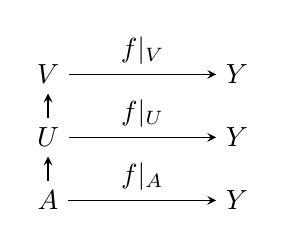
\begin{tikzpicture}[>=stealth, baseline=(U.base)]
\node (V) at (0,1.6) {$V$};
\node (U) at (0,0.8) {$U$};
\node (A) at (0,0)   {$A$};
\node (Y1) at (2.4,1.6) {$Y$};
\node (Y2) at (2.4,0.8) {$Y$};
\node (Y3) at (2.4,0)   {$Y$};
\draw[->] (A) -- (U);
\draw[->] (U) -- (V);
\draw[->] (V) -- node[above]{$f|_{V}$} (Y1);
\draw[->] (U) -- node[above]{$f|_{U}$} (Y2);
\draw[->] (A) -- node[above]{$f|_{A}$} (Y3);
\end{tikzpicture}
\]
由此得到
\[i_{U}\,(f|_{U})^{*}\ =\ (f|_{A})^{*}\,,
\]
\[i_{UV}\,(f|_{V})^{*}\ =\ (f|_{U})^{*}\,.
\]

我们按
\[\check{f}(a)\ =\ [\varphi_{X}\,f^{*}(a)]
\]
定义一个\trHomomorphism
\[\check{f}\colon h(Y)\longrightarrow\check{h}(A)\,.
\]

我们观察到
\[[\varphi_{X}\,f^{*}(a)]\ =\ [\varphi_{U}(f|_{U})^{*}(a)]\ =\ [\varphi_{U}\,i_{UX}\,f^{*}(a)]\,,
\]
从而对一切 $U\in\mathcal{O}_{A}$，
\[\check{f}(a)\ =\ [\varphi_{U}(f|_{U})^{*}(a)]\,.
\]

对 $a\in h(Y)$\footnote{原书印作「$a\in h(U)$」：然 $\check{f}$ 与 $(f|_{U})^{*}$ 之定义域均为 $h(Y)$——$\check{f}\colon h(Y)\to\check{h}(A)$，$(f|_{U})^{*}\colon h(Y)\to h(U)$，$h(U)$ 乃是后者的值域——故应为 $a\in h(Y)$，此处径改。——译者注} 我们计算：
\begin{align*}
\Phi\circ\check{f}(a)\ &=\ i_{U}(f|_{U})^{*}(a)\\
&=\ (f|_{A})^{*}(a)\,,
\end{align*}
于是我们得到交换图
\[
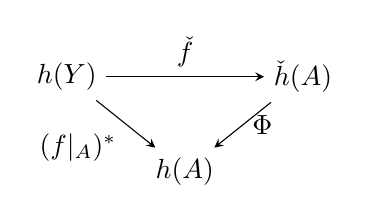
\begin{tikzpicture}[>=stealth, baseline=(hY.base)]
\node (hY) at (0,0) {$h(Y)$};
\node (hA) at (3,0) {$\check{h}(A)$};
\node (hB) at (1.5,-1.2) {$h(A)$};
\draw[->] (hY) -- node[above]{$\check{f}$} (hA);
\draw[->] (hA) -- node[right]{$\Phi$} (hB);
\draw[->] (hY) -- node[below left]{$(f|_{A})^{*}$} (hB);
\end{tikzpicture}
\]
也注意到我们有交换图
\[
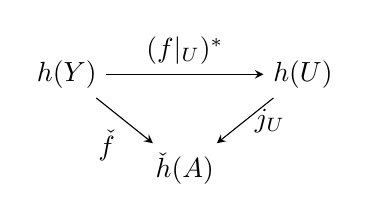
\begin{tikzpicture}[>=stealth, baseline=(hY2.base)]
\node (hY2) at (0,0) {$h(Y)$};
\node (hU) at (3,0) {$h(U)$};
\node (hA2) at (1.5,-1.2) {$\check{h}(A)$};
\draw[->] (hY2) -- node[above]{$(f|_{U})^{*}$} (hU);
\draw[->] (hU) -- node[right]{$j_{U}$} (hA2);
\draw[->] (hY2) -- node[below left]{$\check{f}$} (hA2);
\end{tikzpicture}
\]
其中 $j_{U}(\alpha_{U})=[\varphi_{U}(\alpha_{U})]$。

\begin{proposition}\label{prop:a8-representative}
对每个 $a\in\check{h}(A)$，存在 $U\in\mathcal{O}_{A}$ 与 $\alpha_{U}\in h(U)$
使得 $j_{U}(\alpha_{U})=a$。给定 $\alpha_{U}\in h(U)$ 满足
$j_{U}(\alpha_{U})=0$，则存在 $V\geq U$ 使得 $i_{VU}(\alpha_{U})=0$。
\end{proposition}

\begin{proof}
由前面的讨论，$\check{h}(A)$ 中的每个元素 $a$ 可以写成
$[\varphi_{V}(\gamma)]$ 的形式，其中 $\gamma\in h(V)$，$V\in\mathcal{O}_{A}$
是某个适当的\trNeighborhood。于是
\[j_{V}(\gamma)\ =\ a\,.
\]

假设 $j_{U}(\alpha_{U})=0$。则我们找到 $U_{1}$，$\ldots$、$U_{k}$、
$V_{1}$，$\ldots$、$V_{k}$，满足 $V_{i}\geq U_{i}$ 且 $\alpha_{U_{i}}\in h(U_{i})$，
使得
\begin{equation}\label{eq:a51-relation}
\varphi_{U}(\alpha_{U})\ =\ \sum_{i=1}^{k}\bigl[\varphi_{U_{i}}(\alpha_{U_{i}})\ -\ \varphi_{V_{i}}\,i_{V_{i}U_{i}}(\alpha_{U_{i}})\bigr]\,.
\end{equation}
任取\footnote{原书 \eqref{eq:a51-relation} 有三处径改：求和下标印作「1=1」，疑为「$i=1$」之误植；$\varphi_{V}$ 依上下文（前文引入诸 $V_{i}$、后文计算用 $i_{WV_{l}}$）径补下标作 $\varphi_{V_{i}}$、$i_{V_{i}U_{i}}$；求和项之方括号系译者所增（原书无此括号，去之则语义歧义）。——译者注} $W\in\mathcal{O}_{A}$ 满足
\begin{equation}\label{eq:a52-choice}
W\geq U\,,\ U_{1}\,,\ \ldots\,,\ U_{k}\,,\ V_{1}\,,\ \ldots\,,\ V_{k}\,.
\end{equation}
对 \eqref{eq:a51-relation} 施加 $\sum_{C\leq W}i_{WC}$，我们得到
\begin{align*}
i_{WU}(\alpha_{U})\ &=\ \sum_{l=1}^{k}\Bigl[i_{WU_{l}}(\alpha_{U_{l}})\ -\ i_{WV_{l}}\,i_{V_{l}U_{l}}(\alpha_{U_{l}})\Bigr]\\
&=\ \sum_{l=1}^{k}\Bigl[i_{WU_{l}}(\alpha_{U_{l}})\ -\ i_{WU_{l}}(\alpha_{U_{l}})\Bigr]\ =\ 0\,.
\end{align*}
这对每个满足 \eqref{eq:a52-choice} 的 $W$ 都成立\footnote{原书此二行减项 $i_{WV_{l}}\,i_{V_{l}U_{l}}(\alpha_{U_{l}})$ 印在 $\sum_{l=1}^{k}$ 作用域之外，自由下标 $l$ 悬空、等式「$=0$」推不出，疑为排版漏置；此处径将整个差移入求和号内，并仿 \eqref{eq:a51-relation} 加方括号分组。——译者注}，证明完毕。
\end{proof}


\begin{theorem}\label{thm:a8-check-f-injective}
设 $f\colon X\to Y$ 连续且 $A\subset X$。假设对每个 $U\in\mathcal{O}_{A}$，%
$(f|_{U})^{*}$ 都是\trInjective{}的。则 $\check{f}$ 是\trInjective{}的。
\end{theorem}

\begin{proof}
设 $\check{f}(a)=0$。据 $\check{f}$ 的定义，这意味着对每个 $U\in\mathcal{O}_{A}$ 都有%
\[0\ =\ \bigl[\varphi_{U}(f|_{U})^{*}(a)\bigr]\ =\ j_{U}\bigl((f|_{U})^{*}(a)\bigr)\,.\]
据\cref{prop:a8-representative}，存在 $V\geq U$ 使得
\[0\ =\ i_{VU}\bigl((f|_{U})^{*}(a)\bigr)\,.\]
而 $i_{VU}(f|_{U})^{*}(a)=(f|_{V})^{*}(a)$，从而由 $(f|_{V})^{*}$ 是\trInjective{}的%
可知 $a=0$。
\end{proof}

\begin{corollary}\label{cor:a8-fa-injective}
设 $f\colon X\to Y$ 连续且 $A\subset X$。若 $h$ 在 $A$ 处连续，且对每个%
 $U\in\mathcal{O}_{A}$ 映射 $(f|_{U})^{*}$ 都是\trInjective{}的，则 $(f|_{A})^{*}$ 是%
\trInjective{}的。
\end{corollary}

\begin{proof}
我们有交换图
\[
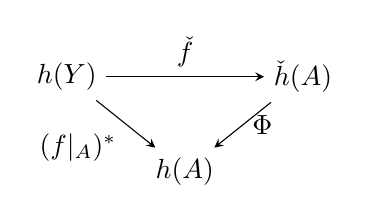
\begin{tikzpicture}[>=stealth, baseline=(cY.base)]
\node (cY) at (0,0) {$h(Y)$};
\node (cA) at (3,0) {$\check{h}(A)$};
\node (cB) at (1.5,-1.2) {$h(A)$};
\draw[->] (cY) -- node[above]{$\check{f}$} (cA);
\draw[->] (cA) -- node[right]{$\Phi$} (cB);
\draw[->] (cY) -- node[below left]{$(f|_{A})^{*}$} (cB);
\end{tikzpicture}
\]
据\cref{thm:a8-check-f-injective}，映射 $\check{f}$ 是\trInjective{}的；据%
\cref{thm:a8-direct-limit-isomorphism}，映射 $\Phi$ 是一个\trIsomorphism。故%
 $(f|_{A})^{*}$ 是\trInjective{}的。
\end{proof}

接下来我们把前面的讨论应用于\trAlexander-\trSpanier{}\trCohomology{}理论。我们请%
读者参阅 E.~\trSpanier{}的原始论文 [202]、E.~\trSpanier{}的书 [203] 以及%
 W.\,S.~\trMassey{}的精彩著作 [149]。

\begin{definition}[{另见 [202]}]\label{def:a8-taut}
设 $X$ 是一个\trTopology{}空间，$A$ 是一个子空间。若对每个系数环 $R$，%
\trAlexander-\trSpanier{}\trCohomology{}函子 $\bar{H}^{i}(\cdot,\,R)$（对每个 $i$）%
都在 $A$ 处连续，我们就称 $A$ 在 $X$ 中是\textbf{\trTaut{}的}（taut）。
\end{definition}

下面这条十分有用的定理归于 E.~\trSpanier，我们请读者参阅 [204]。

\begin{theorem}\label{thm:a8-spanier-tautness}
在下述每一种情形，$A$ 在 $X$ 中都是\trTaut{}的：
\begin{enumerate}
\item[(i)] $A$ 是\trCompact{}的且 $X$ 是\trHausdorff{}的。
\item[(ii)] $A$ 是\trClosed{}的且 $X$ 是\trParacompact{}与\trHausdorff{}的。
\item[(iii)] $A$ 是任意的且 $X$ 中每个开集都是\trParacompact{}与\trHausdorff{}的。
\item[(iv)] $A$ 是一个\trNeighborhoodRetract。
\end{enumerate}
\end{theorem}

于是我们注意到：在\trMetrizable{}空间中每个子集 $A$ 都是\trTaut{}的，从而据%
\cref{thm:a8-direct-limit-isomorphism}
\[
\bar{H}^{*}(A)\ \simeq\ \operatorname*{dir.\,lim}_{\,U\in\mathcal{O}_{A}}\ \bar{H}^{*}(U)\,.
\]
